\subsection{Sol-Gel Synthesis Method}
\noindent This subsection is based on chapter 3 of B. L. Cushing \textit{et al.} review paper \textit{Recent Advances in the Liquid- Phase Synthesis of Inorganic Nanoparticles} \cite{solgel_review}.

In general, sol-gel processing combines small molecules to form a solid material.
This is done using a solution of precursors (the \textit{sol}) that forms a network of bound molecules (the \textit{gel}).
Traditionally, sol-gel processing only referred to the hydrolysis and condensation of alkoxide based precursor such as Si(OEt)$_2$ (tetraethyl orthosilicate), but today it refers to all processes using sol-gel.
The sol-gel synthesis method can be divided into the following six distinct steps.

Step (1): The formation of a stable solution of the alkoxide or solvated metal precursor.

Step (2): The gelation that results in the formation  an oxide- or alcohol-bridged network by polycondensation or polyesterification reactions.
This dramatically increases the viscosity of the solution.

Step (3):  The aging of the cell, also known as syneresis.
In this step, the gel network contracts and expulses the solution from the pores, and the reactions continue until the gel forms a solid mass.

Step (4): The drying of the gel where water and other volatile liquids are removed.
This step is complicated because it fundamentally changes the gel structure.
The drying process consists of four sub-steps: (i) the constant rate period, (ii) the critical point, (iii), the first falling rate period, and (iv) the second falling rate period.
The result is either termed a xerogel, if isolated by thermal evaporation, or an aerogel, if the solvent is extracted under supercritical conditions.

Step (5): Dehydration of the gel using high temperatures.
This removes surface-bound M-OH groups, thus stabilizing against rehydration.

Step (6): The densification and decomposition of the gel.
This makes the gel pores collapse, and all remaining organic species are volatilized.

\subsection{Chemistry of the Sols}

\noindent Using the sol-gel synthesis method, one can produce several types of materials.
One example of such a material is BTO (BaTiO$_3$), which can be made of a mixture of barium sol and titanium sol.
The following paragraph explains the components of these sols and what their functions are.

Barium sol can be made of a mixture of water, EDTA (Ethylenediaminetetraacetic acid), ammonia solution, barium nitrate, and citric acid.
Titanium sol can be made of a mixture of water, citric acid, Titanium isopropoxide, and ammonia solution.
The barium nitrate and the titanium isopropoxide are the sources of the barium and titanium, respectively.
Citric acid is a chelating agent, which means that it reacts with the metal ions to form stable, water-soluable metal complexes.
In the barium solution, EDTA is works as an additional complexing agent.
Finally, since the complex stability depends on the pH, the ammonia solution is used to for adjustments.

\subsection{Profilometer}

\noindent This subsection is based on \textit{nanoScience Instruments} optical profilometry manual \cite{profilometer_manual}.

Profilometers are instruments used to extract topographical data from a surface, e.g. surface morphology, step heights, and surface roughness.
This can either be done using a physical probe or by using light, and is then called stylus profilometey and optical profilometry, respectively.
Stylus profilometers typically gives a height profile along a line, while optical profilometers gives a height profile over an area.
All profilometers is built up of two main parts - a detector and a sample stage.
The detector determines where and how the measurements are taken, while the sample stage holds the sample.

In stylus profilometry, the stylus is physically in contact with the sample surface.
This is schematically shown in figure \autoref{fig:stylus_profilometer}.
At each x-y point, a force feedback loop measures the interactions between the stylus tip and the surface, and the z-value is extracted.
This method provides high vertical resolution, and is good for measuring step heights.
However, as there is physical contact, the surface can potentially be contaminated or damaged.
Also, the stylus tip size and shape influences the measurement, and thus limits the lateral resolution.

\begin{figure}[ht]
    \centering
    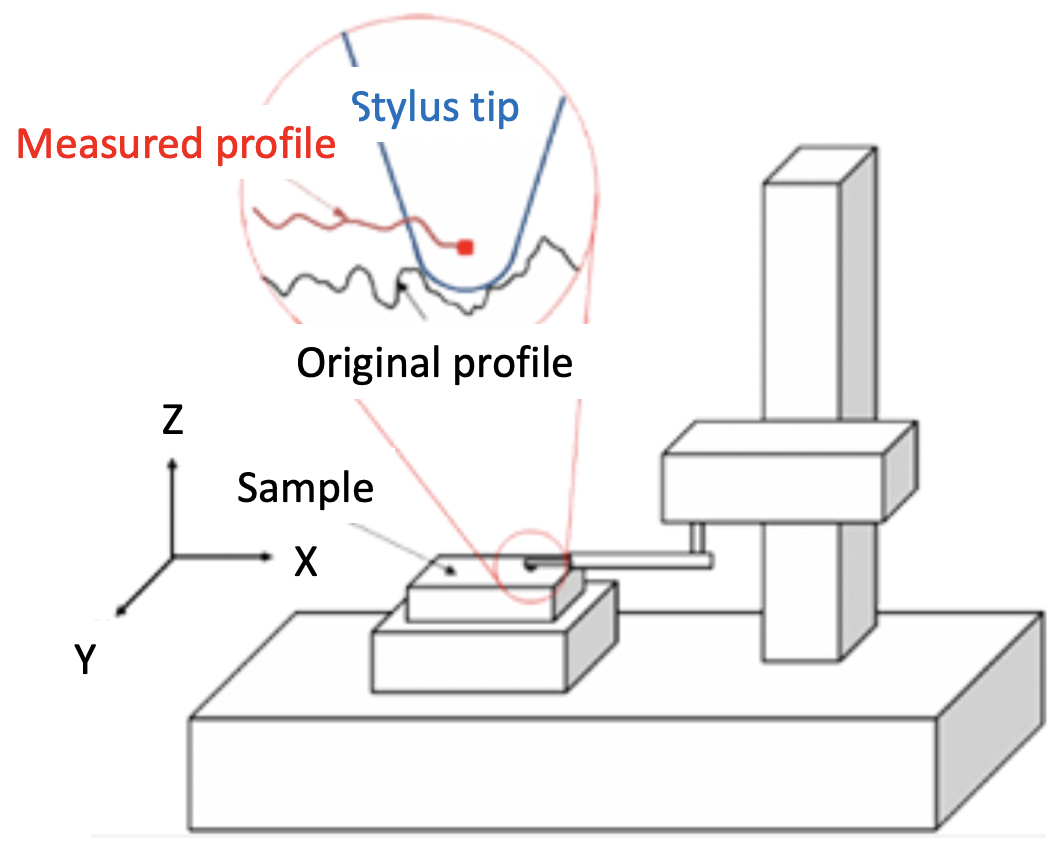
\includegraphics[width=0.45\textwidth]{figures/profilometer.png}
    \caption{Schematic illustration of a stylus profilometer. Figure adapted from \cite{profilometer_manual}.}
    \label{fig:stylus_profilometer}
\end{figure}


\subsection{Scanning Electron Microscope}

% short about the SEM and what contrast it gives.
\noindent The section on SEM is based on Goldstein chapter 1, 2, and 3 \cite{goldstein_scanning_2018}.
Scanning electron microscopes (SEM) are used for sample analysis, and the image contrast is due to the sample composition and topography.
Composition is given on elemental level with energy dispersive X-ray spectroscopy (EDS), or with Z-contrast imaging with backscattered electrons (BSE).
Topography is given primarily with secondary electrons (SE), and partly be achieved with backscattered electrons (BSE).
The Everhart Thornley Detector (ETD) combines data from the SE and BSE detectors to give a better image contrast \cite{T_Everhart_1960}.


% coating or not
SEM samples needs to be conductive, if not electrons will accumulate on the surface and the image will become distorted.
If the sample is not conductive enough, it can be coated with a thin layer of gold or carbon.
If a sample is partly conductive, a lower voltage can be used to get an image without distortion.

% seeing ferro electric domains in SEM
The SEM can be used to see ferroelectric domains structures in a sample, as illustrated in \autoref{fig:ferroelectric_domains_SEM_Hunnestad2019} from \cite{hunnestad_visualizing_2019}.
The image was taken on the SEM APREO at NTNU NanoLab with 1.5 kV and 50 pA, and gives an overview of the domains in the sample.


% insert figure ferroelectric_domains_SEM_Hunnestad2019.jpg
\begin{figure}[ht]
    \centering
    \includegraphics[width=0.45\textwidth]{figures/ferroelectric_domains_SEM_Hunnestad2019.jpg}
    \caption{
        Ferroelectric domains in an $ErMnO_3$ sample.
        The domains are visible as squiggly lighter and darker gray areas in the image.
        Image taken by Hunnestad and published in his master thesis in 2019 \cite{hunnestad_visualizing_2019}.
        Taken on the SEM APREO with EDT, 1.5 kV and 50 pA.
    }
    \label{fig:ferroelectric_domains_SEM_Hunnestad2019}
\end{figure}
